\begin{figure}

\centering

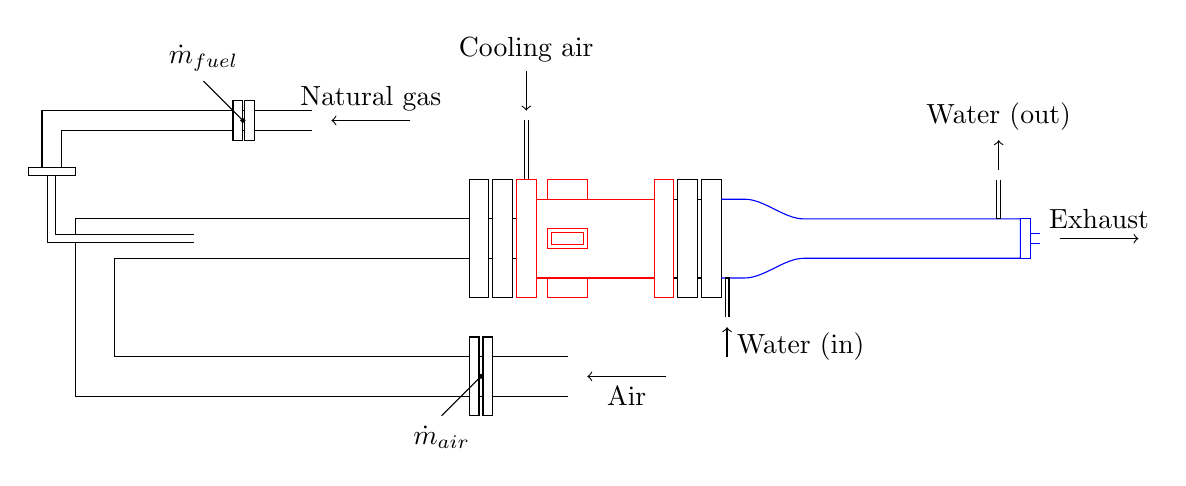
\begin{tikzpicture}[scale=0.5]

%% Air Supply
\draw ( -7, 0.1 ) -- ++( -3, 0 ) -- ++( 0, 0.4 ) -- ++( 10, 0 ) -- ++ ( 0, -1 ) -- ++ ( -9, 0 ) -- ++( 0, -2.5 ) -- ++ ( 9, 0 ) -- ++( 0, -1 ) -- ++( -10, 0 ) -- ++( 0, 3.9 ) -- ++( 3, 0 );
\draw ( 0, -4.5 ) rectangle +( 0.25, 2 );
\draw ( 0.25, -4 ) rectangle +( 0.1, 1 );
\draw ( 0.35, -4.5 ) rectangle +( 0.25, 2 );
\draw ( 0.6, -4 ) -- +( 1.9, 0 );
\draw ( 0.6, -3 ) -- +( 1.9, 0 );

%% Fuel Supply
\draw ( -10, 0.1 ) -- ++( -0.5, 0 ) -- ++( 0, 1.5 ) -- ++( -0.2, 0 ) -- ++( 0, -1.7 ) -- ++( 0.7, 0 );
\draw ( -10, 1.6 ) rectangle ++( -1.2, 0.2 );
\draw ( -10.35, 1.8 ) -- ++( 0, 0.95 ) -- ++( 4.35, 0 );
\draw ( -10.85, 1.8 ) -- ++( 0, 1.45 ) -- ++( 4.85, 0 );
\draw ( -6, 2.5 ) rectangle +( 0.25, 1 );
\draw ( -5.75, 2.75 ) rectangle +( 0.05, 0.5 );
\draw ( -5.7, 2.5 ) rectangle +( 0.25, 1 );
\draw ( -5.45, 2.75 ) -- +( 1.45, 0 );
\draw ( -5.45, 3.25 ) -- +( 1.45, 0 );

%% Cooling air supply
\draw ( 1.5, 3 ) -- ++( 0, -1.5 ) -- ++( -0.1, 0 ) -- ++( 0, 1.5 );

%% Pressure Vessel
% Upstream Flanges
\draw ( 0, -1.5 ) rectangle +( 0.5, 3 );
\draw ( 0.5, -0.5 ) rectangle +( 0.1, 1 );
\draw ( 0.6, -1.5 ) rectangle +( 0.5, 3 );
\draw ( 1.1, -0.5 ) rectangle +( 0.1, 1 );
\draw [red] ( 1.2, -1.5 ) rectangle +( 0.5, 3 );

% Vessel + Windows
\draw [red] ( 1.7, -1 ) rectangle +( 3, 2 );
\draw [red] ( 2, -1 ) rectangle +( 1, -0.5 );
\draw [red] ( 2, 1 ) rectangle +( 1, 0.5 );
\draw [red] ( 2, -0.25 ) rectangle +( 1, 0.5 );
\draw [red] ( 2.1, -0.15 ) rectangle +( 0.8, 0.3 );

% Downstream Flanges
\draw ( 5.9, -1.5 ) rectangle +( 0.5, 3 );
\draw ( 5.8, -1 ) rectangle +( 0.1, 2 );
\draw ( 5.3, -1.5 ) rectangle +( 0.5, 3 );
\draw ( 5.2, -1 ) rectangle +( 0.1, 2 );
\draw [red] ( 4.7, -1.5 ) rectangle +( 0.5, 3 );

%% Exhaust system
\draw [blue] ( 6.4, 1 ) -- ++( 0.6, 0 ) .. controls +( 0.5, 0 ) and +( -0.5, 0 ) .. ++( 1.5, -0.5 ) -- ++( 5.5, 0 ) -- ++( 0, -1 ) -- ++( -5.5, 0 ) .. controls +( -0.5, 0 ) and +( 0.5, 0 ) .. ++( -1.5, -0.5 ) -- ++ ( -0.6, 0 );
\draw [blue] ( 14, -0.5 ) rectangle ++( 0.25, 1 );
\draw [blue] (14.5, 0.125 ) -- ++( -0.25, 0 ) -- ++( 0, -0.25 ) -- ++( 0.25, 0 );

% Water cooling
\draw ( 6.5, -2 ) -- ++( 0, 1 ) -- ++( 0.1, 0 ) -- ++( 0, -1 );
\draw ( 13.5, 1.5 ) -- ++( 0, -1 ) -- ++( -0.1, 0 ) -- ++( 0, 1 );

%% Labels
\draw [->] ( 5, -3.5 ) -- ++( -2, 0 );
\node at ( 4, -3.5 ) [below] {Air};

\draw [->] ( -1.5, 3 ) -- ++( -2, 0 );
\node at ( -2.5, 3 ) [above] {Natural gas};

\draw [->] ( 1.45, 4.25 ) -- ++( 0, -1 );
\node at ( 1.45, 4.25 ) [above] {Cooling air};

\draw [->] ( 6.55, -3 ) -- ++( 0, 0.75 );
\node at ( 6.55, -2.75 ) [right] {Water (in)};

\draw [->] ( 13.45, 1.75 ) -- ++( 0, 0.75 );
\node at ( 13.45, 2.5 ) [above] {Water (out)};

\draw [->] ( 15, 0 ) -- ++( 2, 0 );
\node at ( 16, 0 ) [above] {Exhaust};

\filldraw ( -0.7, -4.5 ) node [below] {\(\dot{m}_{air}\)} -- ++( 1, 1 ) circle ( 0.05 );
\filldraw ( -6.75, 4 ) node [above] {\(\dot{m}_{fuel}\)} -- ++( 1, -1 ) circle ( 0.05 );

\end{tikzpicture}

\caption[Schematic of Test Facility A]{A schematic of the high pressure testing facility where Configuration A was operated is shown. The pressure vessel is outlined in \textcolor{red}{red}, while the water-cooled exhaust section is outlined in \textcolor{blue}{blue}. The locations of the orifice flow meters used to measure the mass flow rates of the preheated air and natural gas fuel are indicated.}

\label{fig:testFacilityA}

\end{figure}

